\documentclass[../main.tex]{subfiles}
\begin{document}
\subsection{Гистограммы и графики плотности распределения}
	\begin{figure}[H]
		\centering
		\begin{tabular}{ccc}
			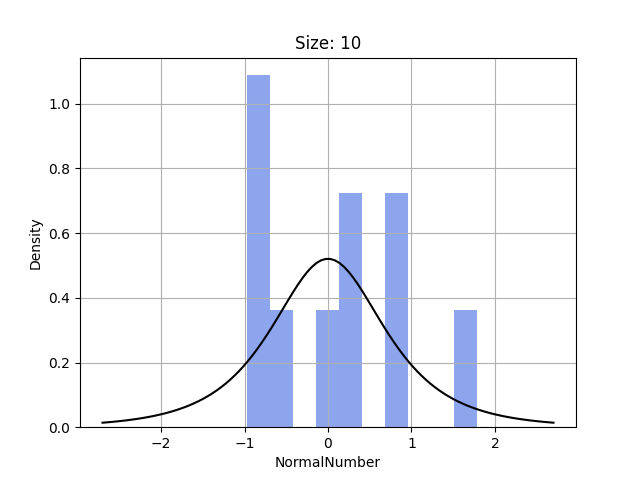
\includegraphics[width=55mm, height =0.25\textheight]{figures/NormalNumber10.png} 
			&
			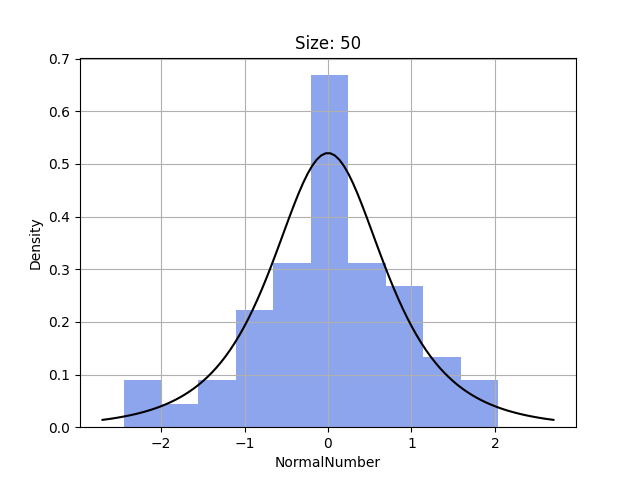
\includegraphics[width=55mm, height =0.25\textheight]{figures/NormalNumber50.png}
			&
			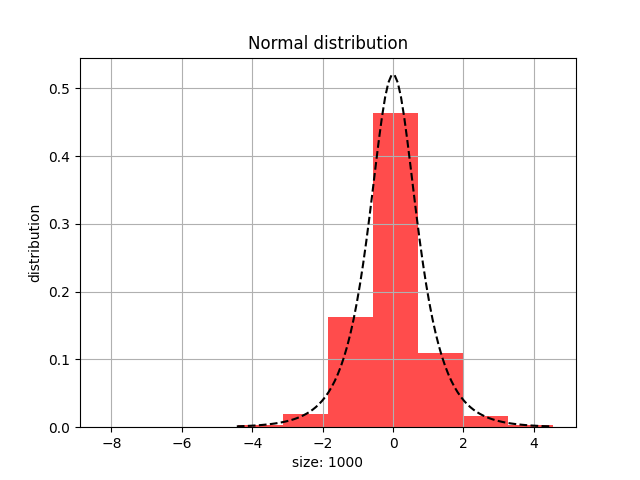
\includegraphics[width=55mm, height =0.25\textheight]{figures/NormalNumber1000.png}
		\end{tabular}
		\caption{Нормальное распределение} 
		\label{fig:normal}
	\end{figure}
	
	\begin{figure}[H]
		\centering
		\begin{tabular}{ccc}
			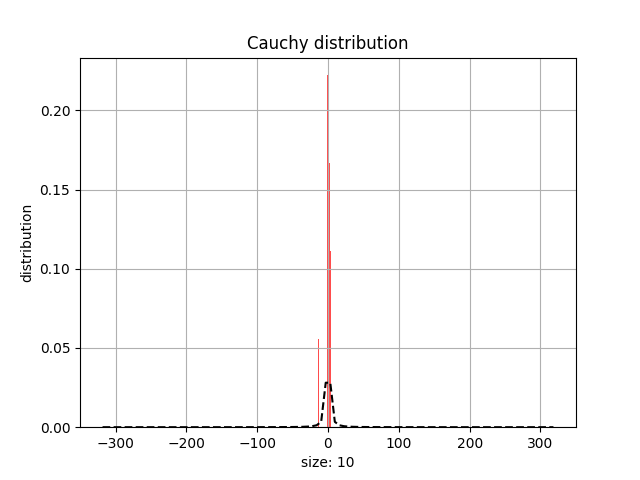
\includegraphics[width=55mm, height =0.25\textheight]{figures/CauchyNumber10.png} 
			&
			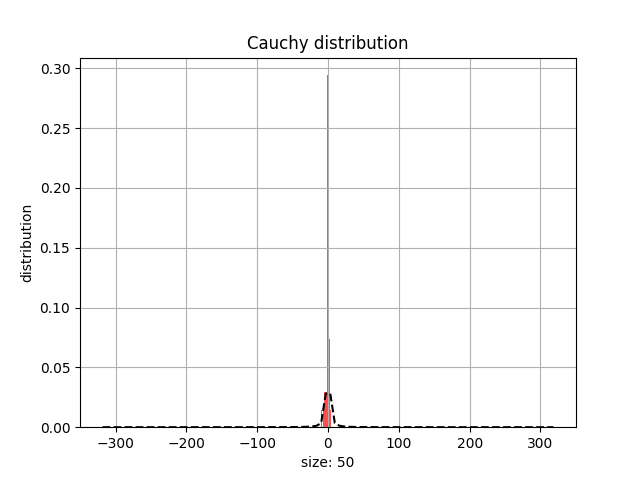
\includegraphics[width=55mm, height =0.25\textheight]{figures/CauchyNumber50.png}
			&
			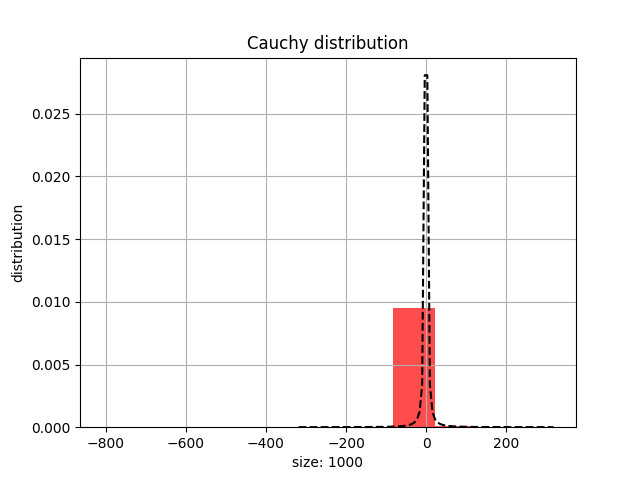
\includegraphics[width=55mm, height =0.25\textheight]{figures/CauchyNumber1000.png}
		\end{tabular}
		\caption{Распределение Коши} 
		\label{fig:normal}
	\end{figure}
	
	\begin{figure}[H]
		\centering
		\begin{tabular}{ccc}
			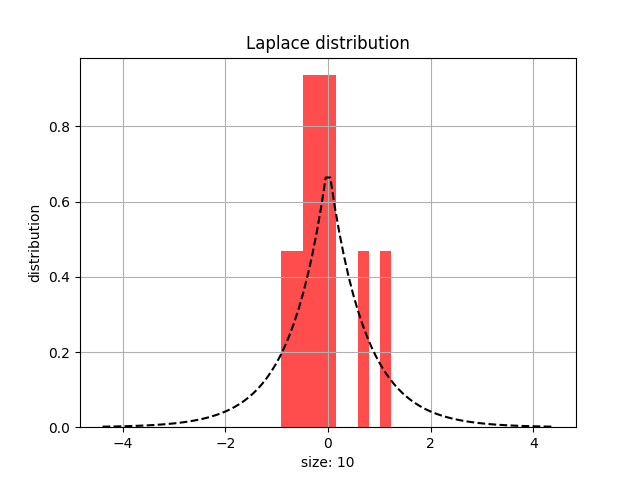
\includegraphics[width=55mm, height =0.25\textheight]{figures/LaplaceNumber10.png} 
			&
			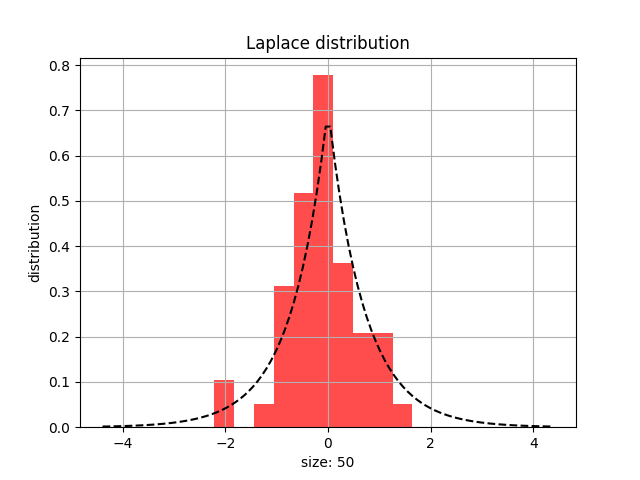
\includegraphics[width=55mm, height =0.25\textheight]{figures/LaplaceNumber50.png}
			&
			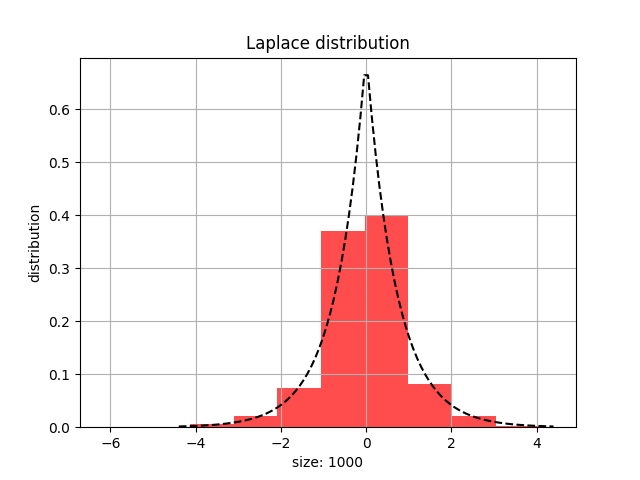
\includegraphics[width=55mm, height =0.25\textheight]{figures/LaplaceNumber1000.png}
		\end{tabular}
		\caption{Распределение Лапласа} 
		\label{fig:normal}
	\end{figure}
	
	\begin{figure}[H]
		\centering
		\begin{tabular}{ccc}
			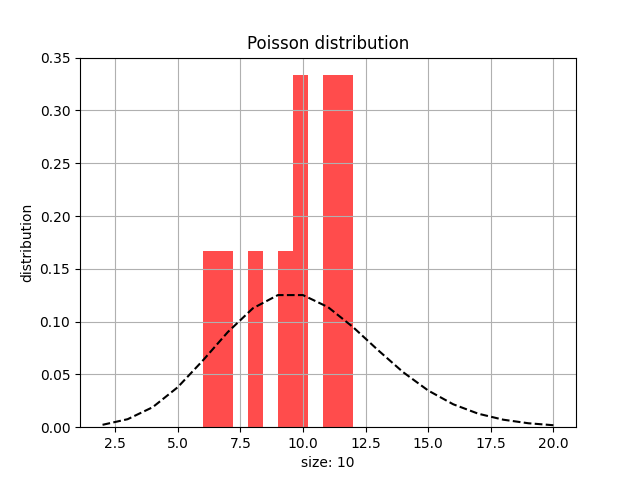
\includegraphics[width=55mm, height =0.25\textheight]{figures/PoissonNumber10.png} 
			&
			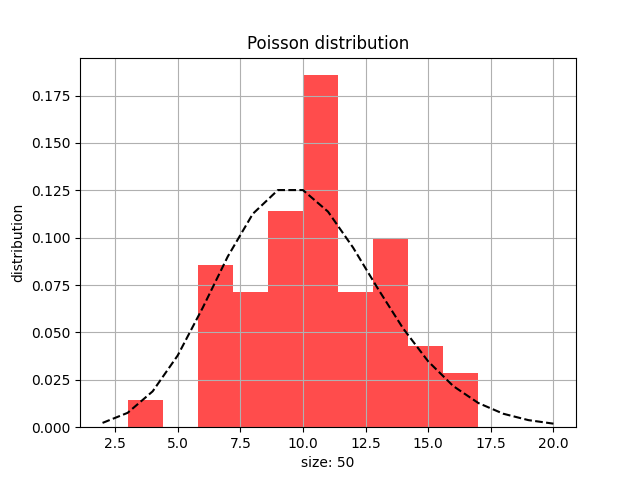
\includegraphics[width=55mm, height =0.25\textheight]{figures/PoissonNumber50.png}
			&
			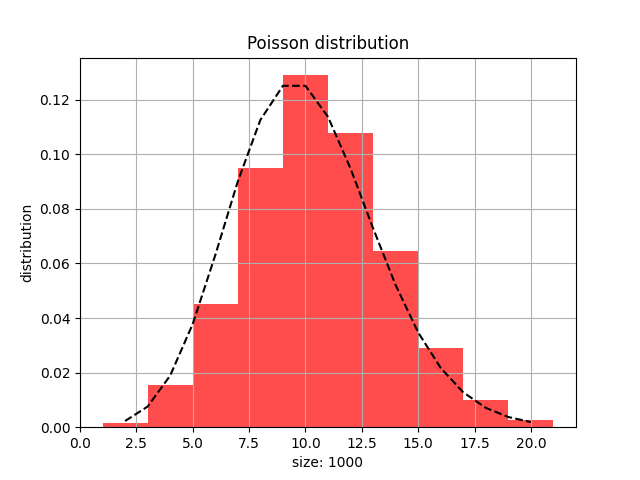
\includegraphics[width=55mm, height =0.25\textheight]{figures/PoissonNumber1000.png}
		\end{tabular}
		\caption{Распределение Пауссона} 
		\label{fig:normal}
	\end{figure}
	
	\begin{figure}[H]
		\centering
		\begin{tabular}{ccc}
			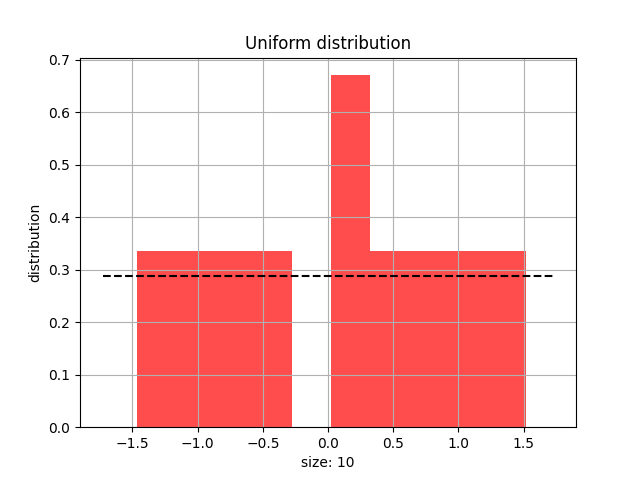
\includegraphics[width=55mm, height =0.25\textheight]{figures/UniformNumber10.png} 
			&
			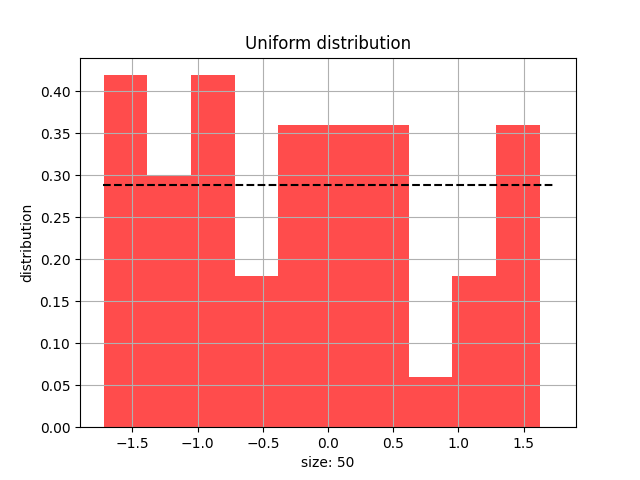
\includegraphics[width=55mm, height =0.25\textheight]{figures/UniformNumber50.png}
			&
			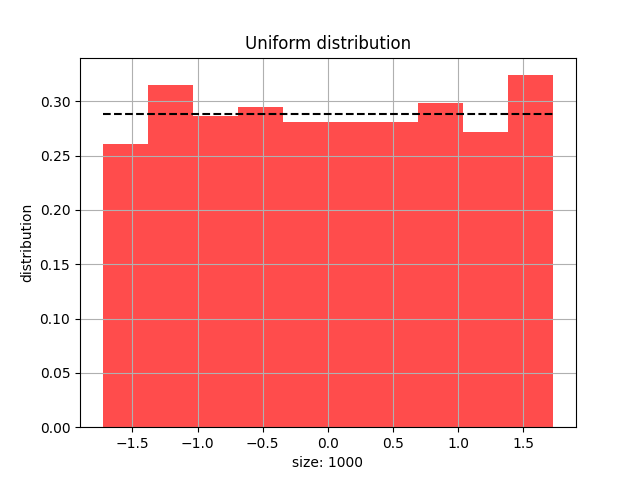
\includegraphics[width=55mm, height =0.25\textheight]{figures/UniformNumber1000.png}
		\end{tabular}
		\caption{Равномерное распределение} 
		\label{fig:normal}
	\end{figure}
	
	\subsection{Характеристики положения и рассеяния}
	
	\begin{table}[H]
    \centering
    \begin{tabular}{|l||c|c|c|c|c|}
        \hline
        & $\overline{x}$ & $med x$ & $z_R$ & $z_Q$ & $z_{tr}$\\\hline\hline
        n=10 & & & & &\\\hline
        $E(z)$ & 0.002014 & 0.00019 & -0.009066 & 0.319223 & 0.281011\\\hline
        $D(z)$ & 0.091659 & 0.135694 & 0.170231 & 0.117384 & 0.107012\\\hline
        E(z) \pm \sqrt{D(z)} & [0.30476; & [0.368555; & [0.40352; & [0.66183; & [0.60813;\\
		&  -0.30073] & -0.368175] & -0.42165] & -0.02339] & -0.04611] \\\hline
		\widehat{E}(z) & 0 & 0 & 0 & 0 & 0\\\hline
        n=100 & & & & &\\\hline
        $E(z)$ & 0.00417 & 0.007801 & -0.006201 & 0.020803 & 0.0326\\\hline
        $D(z)$ & 0.009688 & 0.015677 & 0.097562 & 0.012515 & 0.011869\\\hline
        E(z) \pm \sqrt{D(z)} & [0.10259; & [0.13300; & [0.30614; & [0.13267; & [0.14154;\\
		& -0.09425] & -0.11740] & -0.31855] & -0.09106] & -0.07634] \\\hline
		\widehat{E}(z) & 0 & 0 & 0 & 0 & 0\\\hline
        n=1000 & & & & &\\\hline
        $E(z)$ & -0.001895 & -0.001776 & -0.004071 & 0.000663 & 0.001123\\\hline
        $D(z)$ & 0.00103 & 0.001524 & 0.058838 & 0.001297 & 0.001176\\\hline
        E(z) \pm \sqrt{D(z)} & [0.03019; & [0.03726; & [0.23849; & [0.03667; & [0.03541; \\
		&  -0.03398] & -0.04081] & -0.24663] & -0.03535] & -0.03316] \\\hline
		\widehat{E}(z) & 0.0 & 0.0 & 0 & 0.0 & 0.0\\\hline
    \end{tabular}
    \caption{Нормальное распределение}
    \label{tab:normal}
    \end{table}
    
    \begin{table}[H]
    \centering
    \begin{tabular}{|l||c|c|c|c|c|}
        \hline
        & $\overline{x}$ & $med x$ & $z_R$ & $z_Q$ & $z_{tr}$\\\hline\hline
        n=10 & & & & &\\\hline
        $E(z)$ & -0.067513 & -0.025744 & -0.288092 & 1.179057 & 0.689997\\\hline
        $D(z)$ & 846.317773 & 0.326448 & 20847.646823 & 9.225355 & 1.903638\\\hline
        E(z) \pm \sqrt{D(z)} & [29.02402; & [0.54561; & [144.09905; & [4.21638; & [2.06972; \\
		&  -29.15905] & -0.59710] & -144.67523] & -1.85826] & -0.68972] \\\hline
		\widehat{E}(z) & - & 0 & - & - & -\\\hline
        n=100 & & & & &\\\hline
        $E(z)$ & -7.796638 & 1e-06 & -389.028757 & 0.032576 & 0.039317\\\hline
        $D(z)$ & 59941.059759 & 0.024992 & 149818127.185183 & 0.051438 & 0.026913\\\hline
        E(z) \pm \sqrt{D(z)} & [237.03199; & [0.15808; & [11850.99277; & [0.25937; & [0.20336; \\
		&  -252.62527] & -0.15808] & -12629.05029] & -0.19422] & -0.12473] \\\hline
		\widehat{E}(z) & - & 0 & - & 0 & 0\\\hline
        n=1000 & & & & &\\\hline
        $E(z)$ & 0.170678 & -0.000289 & 106.285035 & 0.002004 & 0.003382\\\hline
        $D(z)$ & 1741.899548 & 0.002541 & 434098418.982262 & 0.004821 & 0.002599\\\hline
        E(z) \pm \sqrt{D(z)} & [41.90674; & [0.05011; & [20941.31368; & [0.07143; & [0.05436; \\
		&  -41.56539] & -0.05069] & -20728.74361] & -0.06742] & -0.047598] \\\hline
		\widehat{E}(z) & - & 0.0 & - & 0.0 & 0.0\\\hline
    \end{tabular}
    \caption{Распределение Коши}
    \label{tab:normal}
    \end{table}
    
    \begin{table}[H]
    \centering
    \begin{tabular}{|l||c|c|c|c|c|}
        \hline
        & $\overline{x}$ & $med x$ & $z_R$ & $z_Q$ & $z_{tr}$\\\hline\hline
        n=10 & & & & &\\\hline
        $E(z)$ & -0.027681 & -0.015697 & -0.037881 & 0.27275 & 0.209486\\\hline
        $D(z)$ & 0.104043 & 0.072293 & 0.451381 & 0.119055 & 0.079919\\\hline
        E(z) \pm \sqrt{D(z)} & [0.29487; & [0.25317; & [0.63396; & [0.61779; & [0.49218;\\
		&  -0.35023] & -0.28457] & -0.70972] & -0.07229] & -0.07321] \\\hline
		\widehat{E}(z) & 0 & 0 & 0 & 0 & 0\\\hline
        n=100 & & & & &\\\hline
        $E(z)$ & -0.001001 & -0.000606 & 0.007335 & 0.010771 & 0.018518\\\hline
        $D(z)$ & 0.009797 & 0.00542 & 0.423671 & 0.009122 & 0.005824\\\hline
        E(z) \pm \sqrt{D(z)} & [0.09797; & [0.07301; & [0.65823; & [0.10628; & [0.09483; \\
		&  -0.09998] & -0.07422] & -0.64356] & -0.08473] & -0.05779] \\\hline
		\widehat{E}(z) & 0.0 & 0.0 & 0 & 0 & 0.0\\\hline
        n=1000 & & & & &\\\hline
        $E(z)$ & -0.00085 & -0.000406 & 0.021226 & 0.001039 & 0.001315\\\hline
        $D(z)$ & 0.001037 & 0.000518 & 0.412182 & 0.001052 & 0.000621\\\hline
        E(z) \pm \sqrt{D(z)} & [0.03135; & [0.02235; & [0.66324; & [0.03347; & [0.02623; \\
		& -0.03305] & -0.02316] & -0.62078] & -0.03139] & -0.02360] \\\hline
		\widehat{E}(z) & 0.0 & 0.0 & 0 & 0.0 & 0.0\\\hline
    \end{tabular}
    \caption{Распределение Лапласа}
    \label{tab:normal}
    \end{table}
	
	\begin{table}[H]
    \centering
    \begin{tabular}{|l||c|c|c|c|c|}
        \hline
        & $\overline{x}$ & $med x$ & $z_R$ & $z_Q$ & $z_{tr}$\\\hline\hline
        n=10 & & & & &\\\hline
        $E(z)$ & 10.0243 & 9.863 & 10.358 & 10.978 & 10.792167\\\hline
        $D(z)$ & 0.93652 & 1.399231 & 1.806836 & 1.319516 & 1.174278\\\hline
        E(z) \pm \sqrt{D(z)} & [10.99203; & [11.04589; & [11.70218; & [12.12670; & [11.87580; \\
		&  9.0565] & 8.68010] & 9.01381] & 9.82929] & 9.70852] \\\hline
		\widehat{E}(z) & 10^{+1}_{-1} & 10^{+1}_{-1} & 10^{+2}_{-2} & 10^{+2}_{-2} & 10^{+2}_{-2}\\\hline
        n=100 & & & & &\\\hline
        $E(z)$ & 9.99245 & 9.8735 & 10.9415 & 9.9555 & 9.9344\\\hline
        $D(z)$ & 0.099154 & 0.189748 & 0.994328 & 0.14777 & 0.115515\\\hline
        E(z) \pm \sqrt{D(z)} & [10.30733; & [10.30910; & [11.93865; & [10.33990; & [10.27427; \\
		&  9.67756] & 9.43789] & 9.94434] & 9.57109] & 9.59452] \\\hline
		\widehat{E}(z) & 10^{+1}_{-1} & 10^{+1}_{-1} & 10^{+2}_{-2} & 10^{+1}_{-1} & 10^{+1}_{-1}\\\hline
        n=1000 & & & & &\\\hline
        $E(z)$ & 9.998721 & 9.997 & 11.6155 & 9.996 & 9.866072\\\hline
        $D(z)$ & 0.010014 & 0.002991 & 0.65991 & 0.001984 & 0.011422\\\hline
        E(z) \pm \sqrt{D(z)} & [10.09879; & [10.05169; & [12.42784; & [10.04054; & [9.97294; \\
		&  9.89865] & 9.94230] & 10.80315] & 9.95145] & 9.75919] \\\hline
		\widehat{E}(z) & 10^{+1}_{-1} & 10^{+1}_{-1} & 10^{+2}_{-2} & 10^{+1}_{-1} & 10^{+1}_{-1}\\\hline
    \end{tabular}
    \caption{Распределение Пуасона}
    \label{tab:normal}
    \end{table}
    
    \begin{table}[H]
    \centering
    \begin{tabular}{|l||c|c|c|c|c|}
        \hline
        & $\overline{x}$ & $med x$ & $z_R$ & $z_Q$ & $z_{tr}$\\\hline\hline
        n=10 & & & & &\\\hline
        $E(z)$ & -0.010227 & -0.010992 & -0.012102 & 0.301643 & 0.305763\\\hline
        $D(z)$ & 0.100166 & 0.228273 & 0.044863 & 0.133498 & 0.157228\\\hline
        E(z) \pm \sqrt{D(z)} & [0.30626; & [0.46678; & [0.19970; & [0.66701; & [0.70228; \\
		&  -0.32671] & -0.48877] & -0.22391] & -0.06373] & -0.09075] \\\hline
		\widehat{E}(z) & 0 & 0 & 0 & 0 & 0\\\hline
        n=100 & & & & &\\\hline
        $E(z)$ & 0.008576 & 0.010706 & 0.000276 & 0.028335 & 0.046755\\\hline
        $D(z)$ & 0.010119 & 0.029637 & 0.000541 & 0.014519 & 0.020428\\\hline
        E(z) \pm \sqrt{D(z)} & [0.10916; & [0.18286; & [0.02353; & [0.14882; & [0.18968; \\
		&  -0.09201] & -0.16144] & -0.02298] & -0.09215] & -0.09617] \\\hline
		\widehat{E}(z) & 0 & 0 & 0.0 & 0 & 0\\\hline
        n=1000 & & & & &\\\hline
        $E(z)$ & 0.000198 & -0.000121 & -0.0001 & 0.002624 & 0.003752\\\hline
        $D(z)$ & 0.000955 & 0.003052 & 7e-06 & 0.001475 & 0.001917\\\hline
        E(z) \pm \sqrt{D(z)} & [0.03110; & [0.05512; & [0.00254; & [0.04102; & [0.04753 ;\\
		& -0.03070] & -0.05536] & -0.00274] & -0.03578] & -0.04003] \\\hline
		\widehat{E}(z) & 0.0 & 0.0 & 0.00 & 0.0 & 0.0\\\hline
    \end{tabular}
    \caption{Нормальное распределение}
    \label{tab:normal}
    \end{table}
	
	\subsection{Боксплот Тьюки}
	
	\begin{figure}[H]
        \centering
        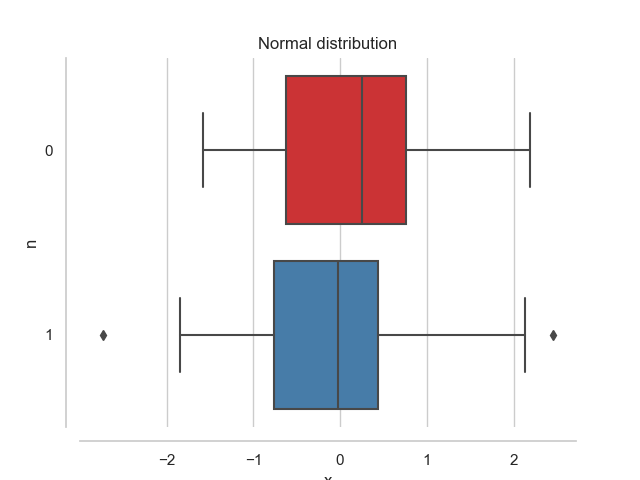
\includegraphics[scale=0.8]{figures/NormalBoxplot.png}
        \caption{Нормальное распределение}
        \label{fig:normal}
    \end{figure}
    
    \begin{figure}[H]
        \centering
        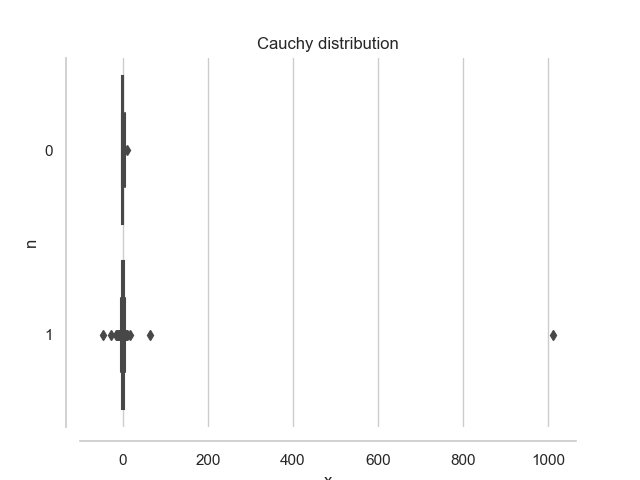
\includegraphics[scale=0.8]{figures/CauchyBoxplot.png}
        \caption{Распределение Коши}
        \label{fig:normal}
    \end{figure}
    
    \begin{figure}[H]
        \centering
        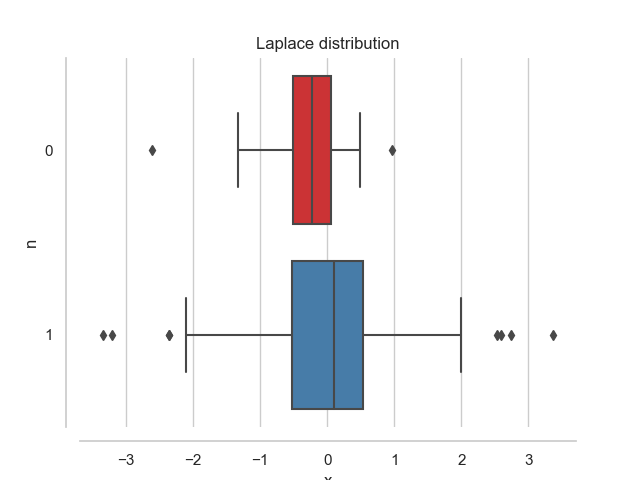
\includegraphics[scale=0.8]{figures/LaplaceBoxplot.png}
        \caption{Распределение Лапласа}
        \label{fig:normal}
    \end{figure}
    
     \begin{figure}[H]
        \centering
        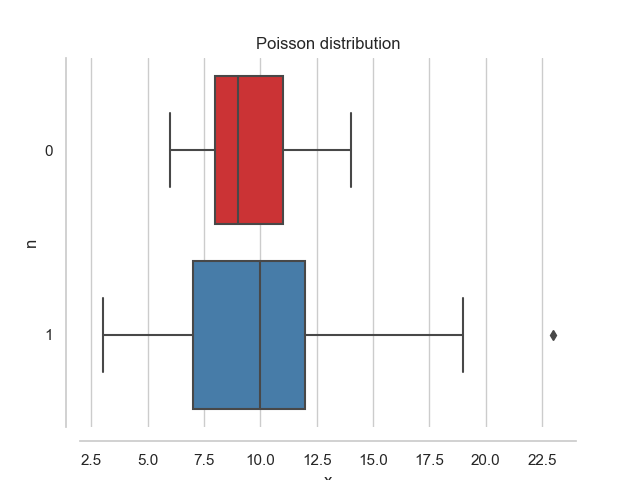
\includegraphics[scale=0.8]{figures/PoissonBoxplot.png}
        \caption{Распределение Пуассона}
        \label{fig:normal}
    \end{figure}
    
    \begin{figure}[H]
        \centering
        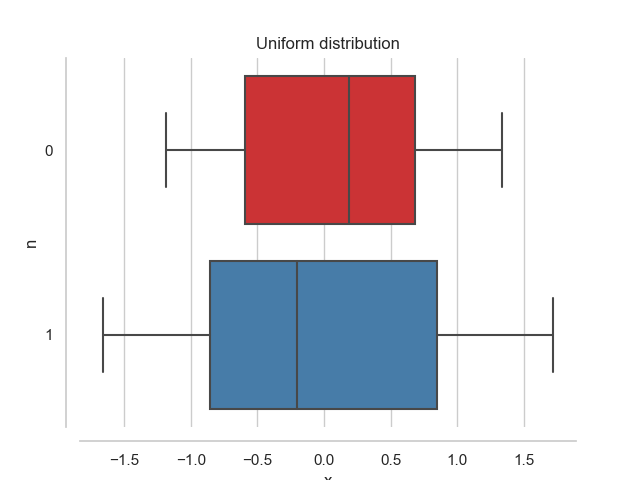
\includegraphics[scale=0.8]{figures/UniformBoxplot.png}
        \caption{Равномерное распределение}
        \label{fig:normal}
    \end{figure}
    
    \subsection{Доля выбросов}
    \begin{table}[H]
	\centering
	\begin{tabular}{|l|c|c|}
		\hline
		Выборка & Доля выбросов	\\\hline
		\hline
		Normal n = 20 & 0.02585 \\\hline
		Normal n = 100 & 0.00989 \\\hline
		Cauchy n = 20 & 0.15075 \\\hline
		Cauchy n = 100 & 0.15655 \\\hline
		Laplace n = 20 & 0.0687 \\\hline
		Laplace n = 100 & 0.06348 \\\hline
		Poisson n = 20 & 0.02355 \\\hline
		Poisson n = 100 & 0.00993 \\\hline
		Uniform n = 20 & 0.0027\\\hline
		Uniform n = 100 & 0 \\\hline
	\end{tabular}
	\caption{Практическая доля выбросов}
    \end{table}
    
    \subsection{Теоретическая вероятность выбросов}
    
    \begin{table}[H]
	\centering
	\begin{tabular}{|l|c|c|c|c|c|}
		\hline
		Распределение & $Q_1^T$	& $Q_3^T$ & $X_1^T$ & $X_2^T$ & $P_B^T$\\\hline
		\hline
		Нормальное & -0.674 & 0.674 & -2.698 &  2.698 & 0.007\\\hline
		Коши & -1 & 1 & -4 & 4 & 0.156\\\hline
		Лапласа & -0.490 & 0.490 & -1.961 & 1.961 & 0.063\\\hline
		Пуассона & 8 & 12 & 2 & 18 & 0.008\\\hline
		Равномерное & -0.866 & 0.866 & -3.464 & 3.464 & 0\\\hline
	\end{tabular}
	\caption{Теоретическая вероятность выбросов}
    \end{table}
    
    \subsection{Эмпирическая функция распределения}
    
    \begin{figure}[H]
        \centering
        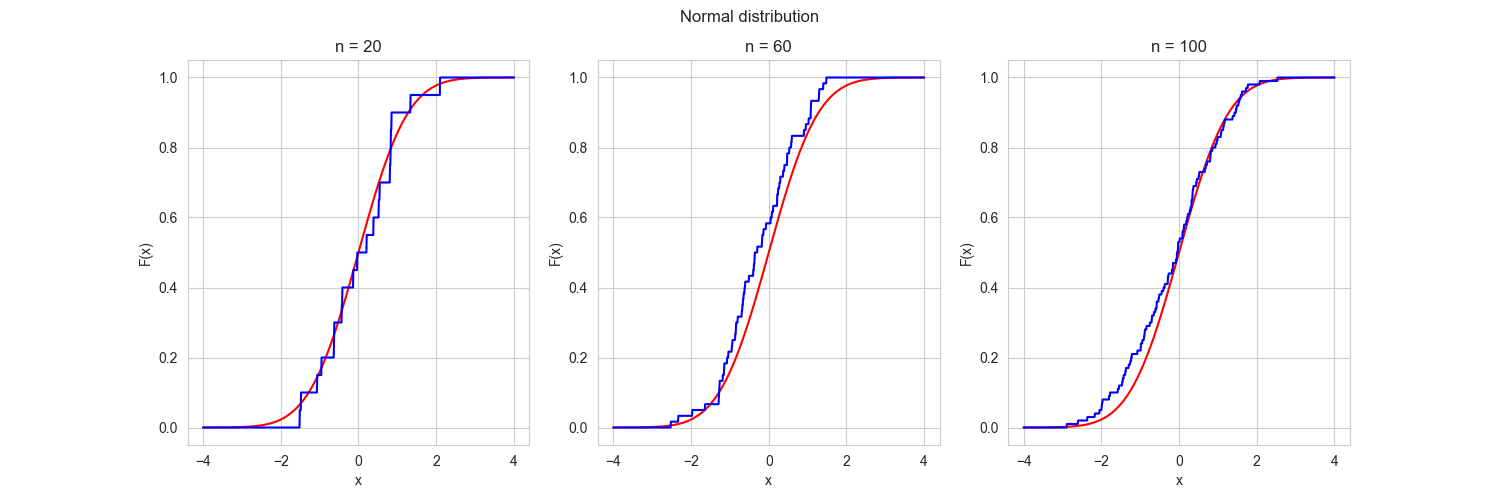
\includegraphics[scale=0.5]{figures/NormalEmpirical.png}
        \caption{Нормальное распределение}
        \label{fig:normal}
    \end{figure}
    
    \begin{figure}[H]
        \centering
        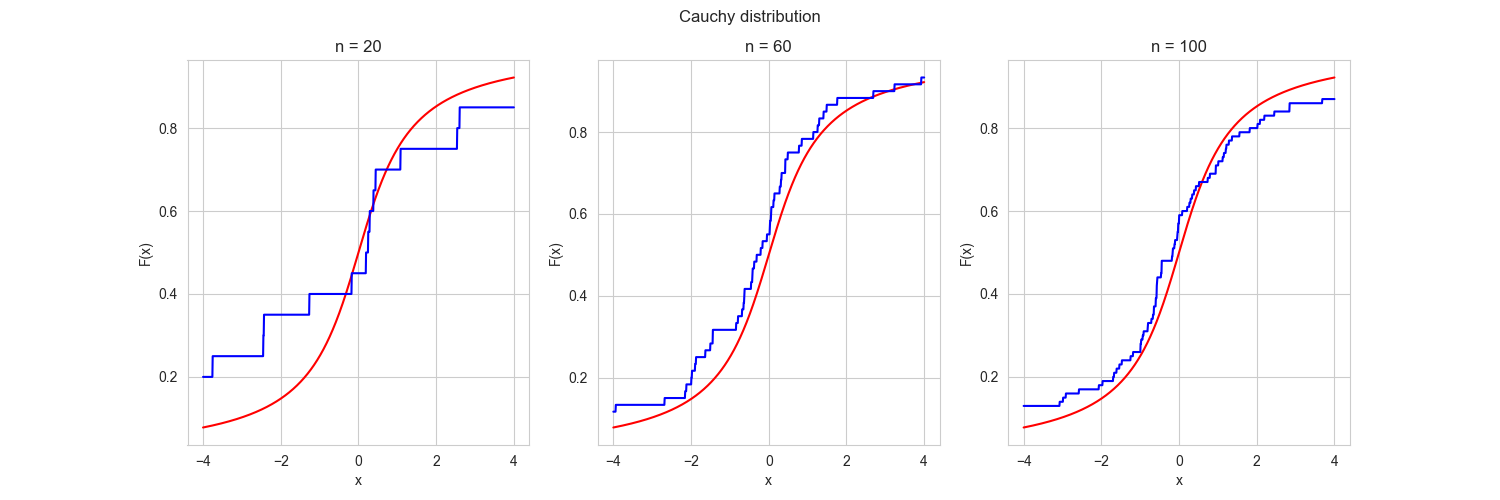
\includegraphics[scale=0.5]{figures/CauchyEmpirical.png}
        \caption{Распределение Коши}
        \label{fig:normal}
    \end{figure}
    
    \begin{figure}[H]
        \centering
        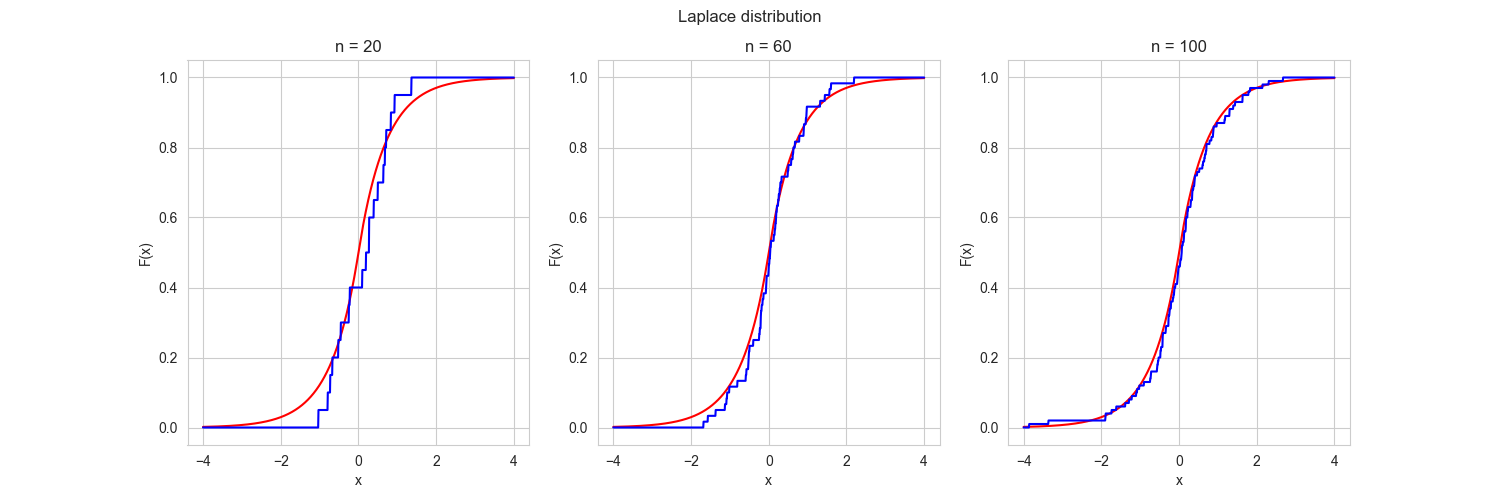
\includegraphics[scale=0.5]{figures/LaplaceEmpirical.png}
        \caption{Распределение Лапласа}
        \label{fig:normal}
    \end{figure}
    
     \begin{figure}[H]
        \centering
        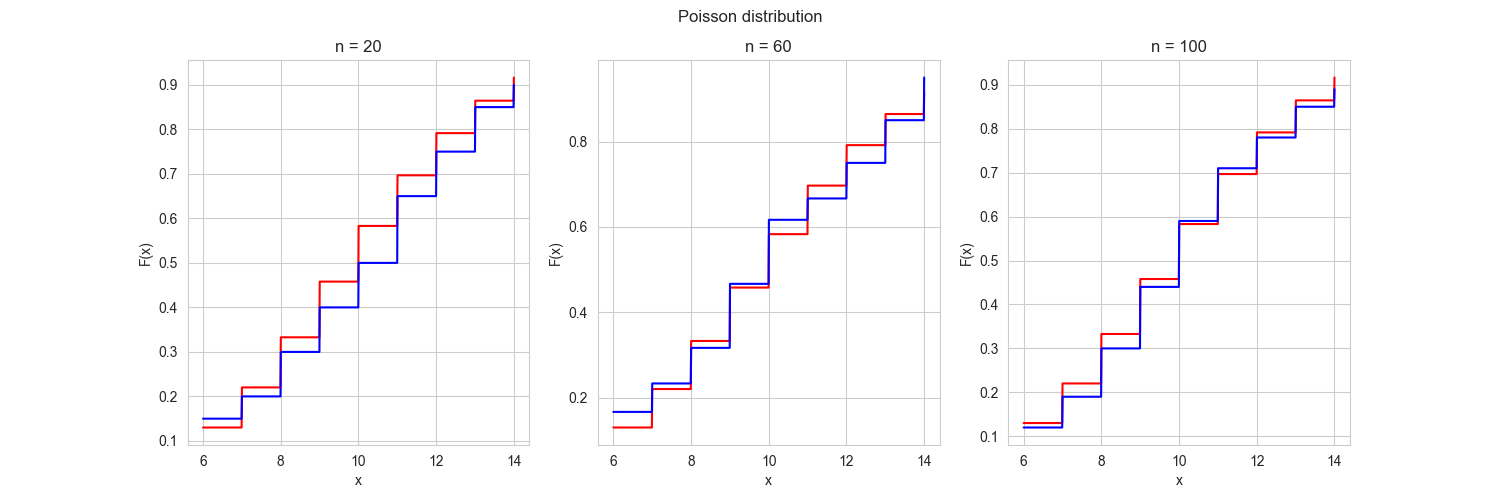
\includegraphics[scale=0.5]{figures/PoissonEmpirical.png}
        \caption{Распределение Пуассона}
        \label{fig:normal}
    \end{figure}
    
    \begin{figure}[H]
        \centering
        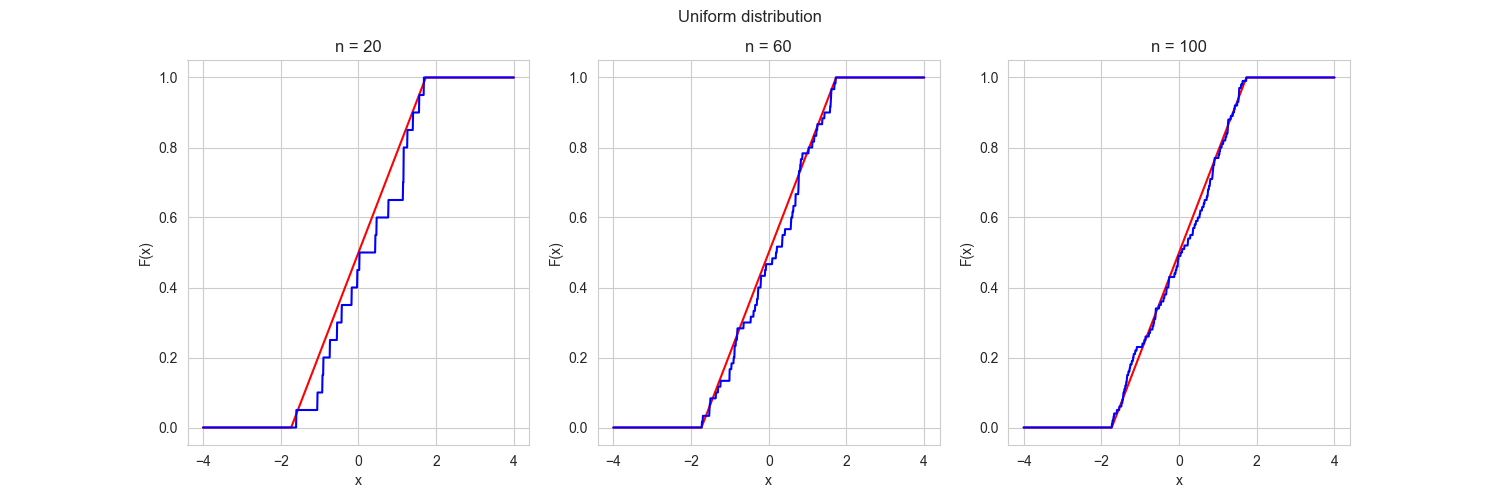
\includegraphics[scale=0.5]{figures/UniformEmpirical.png}
        \caption{Равномерное распределение}
        \label{fig:normal}
    \end{figure}
    
    \subsection{Ядерные оценки плотности распределения}
    
    \begin{figure}[H]
        \centering
        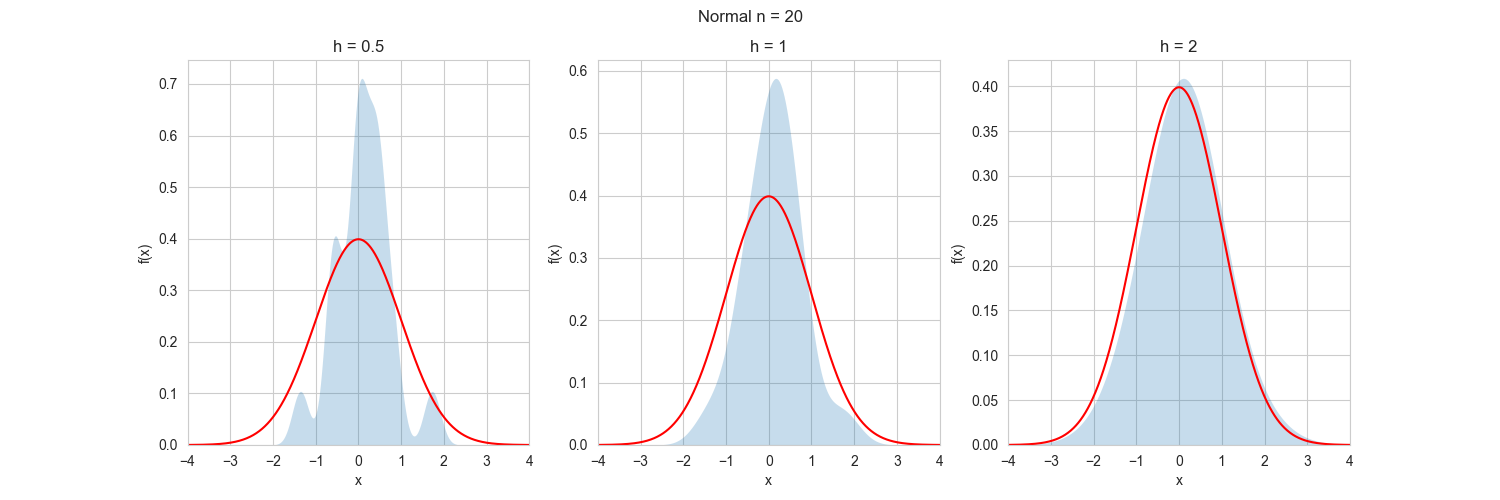
\includegraphics[scale=0.5]{figures/NormalNuclear20.png}
        \caption{Нормальное распределение, n = 20}
        \label{fig:normal}
    \end{figure}
    
    \begin{figure}[H]
        \centering
        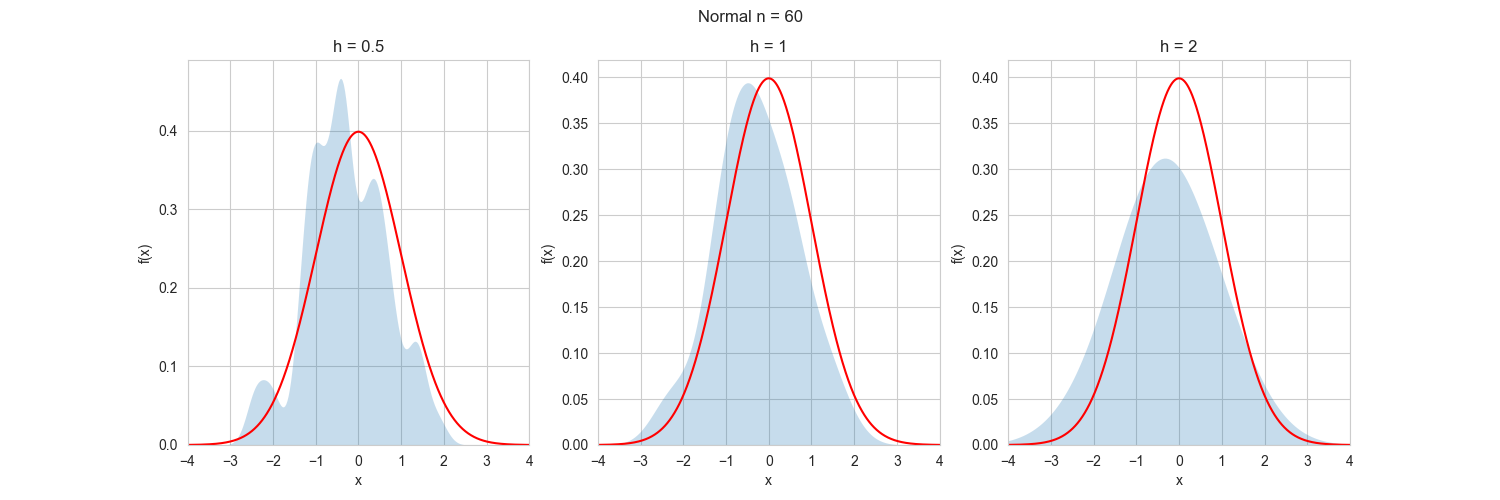
\includegraphics[scale=0.5]{figures/NormalNuclear60.png}
        \caption{Нормальное распределение, n = 60}
        \label{fig:normal}
    \end{figure}
    
    \begin{figure}[H]
        \centering
        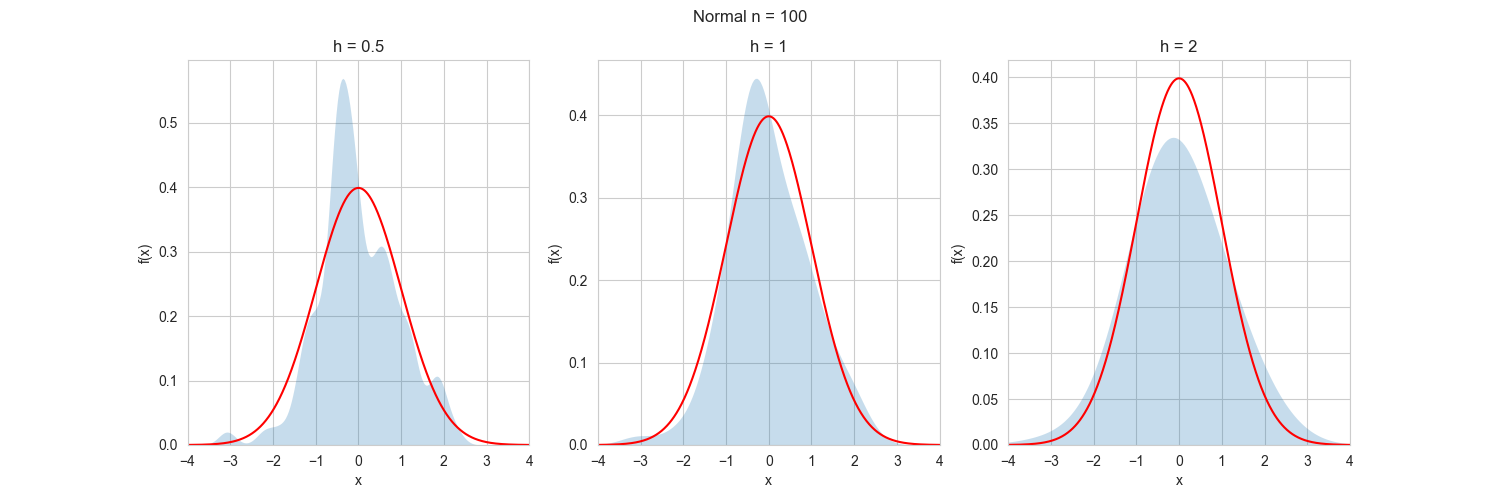
\includegraphics[scale=0.5]{figures/NormalNuclear100.png}
        \caption{Нормальное распределение, n = 100}
        \label{fig:normal}
    \end{figure}
    
    \begin{figure}[H]
        \centering
        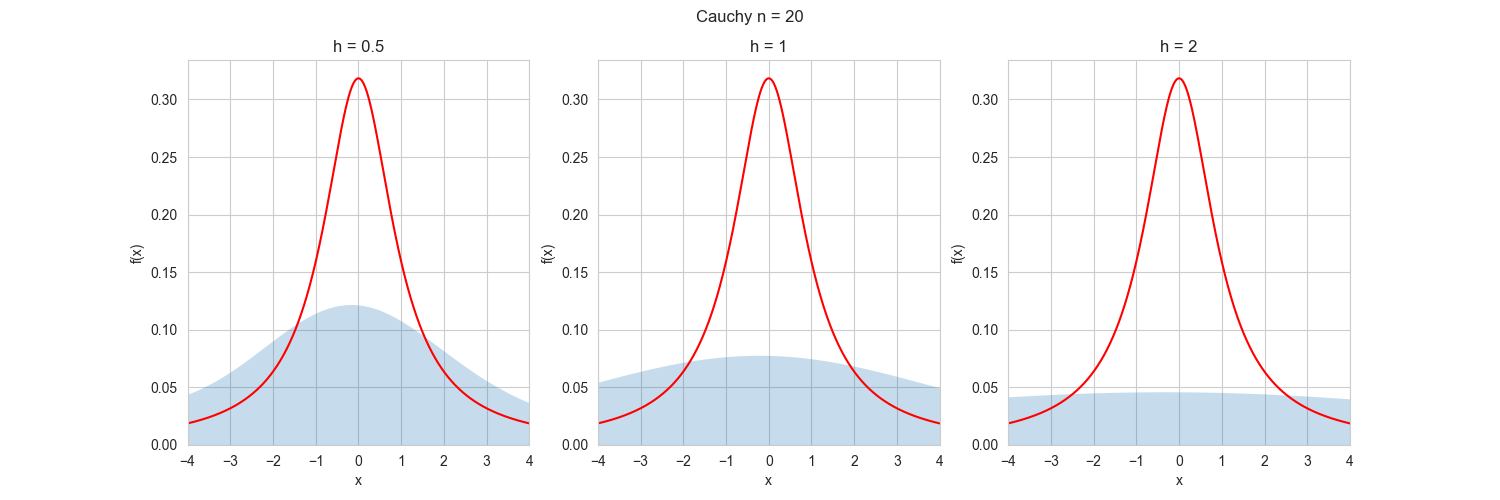
\includegraphics[scale=0.5]{figures/CauchyNuclear20.png}
        \caption{Распределение Коши, n = 20}
        \label{fig:normal}
    \end{figure}
    
    \begin{figure}[H]
        \centering
        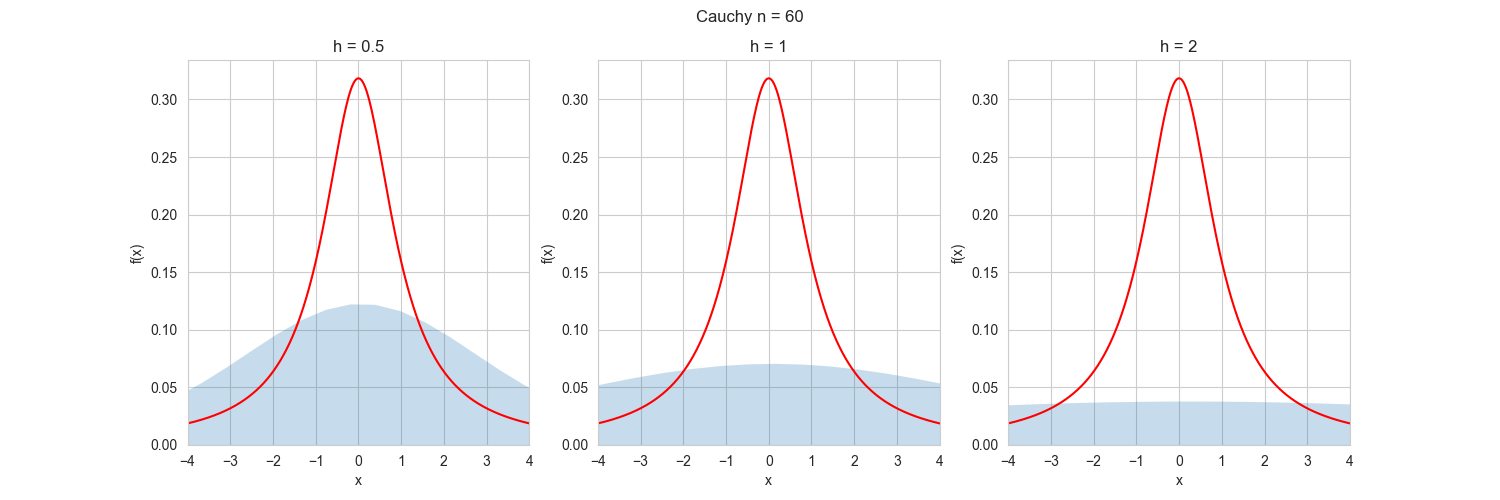
\includegraphics[scale=0.5]{figures/CauchyNuclear60.png}
        \caption{Распределение Коши, n = 60}
        \label{fig:normal}
    \end{figure}
    
    \begin{figure}[H]
        \centering
        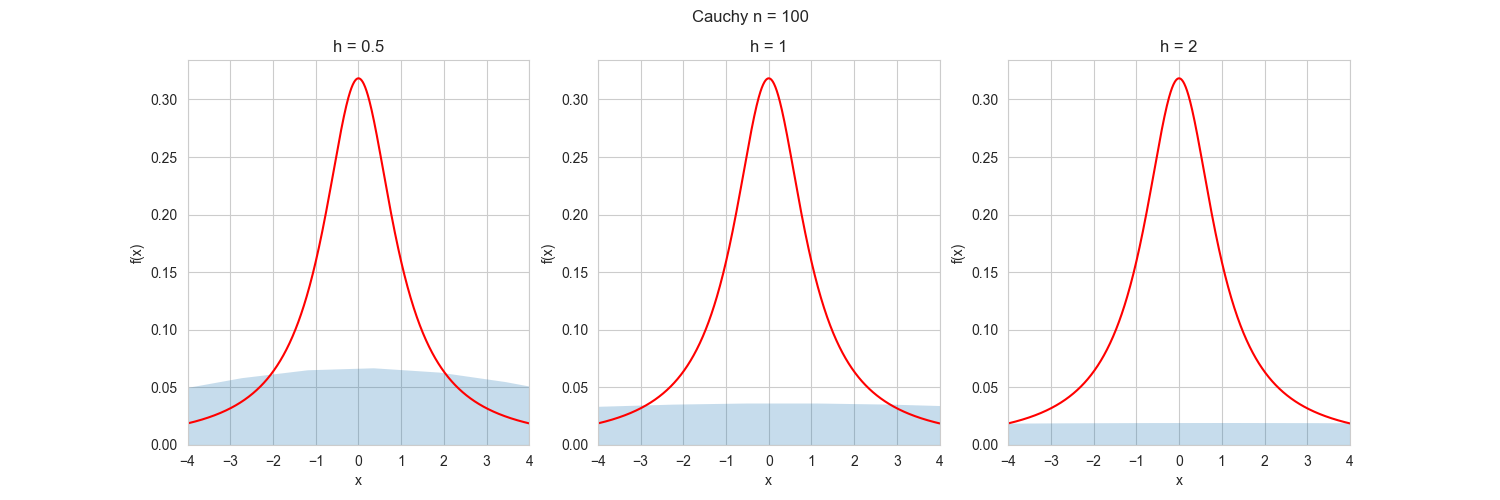
\includegraphics[scale=0.5]{figures/CauchyNuclear100.png}
        \caption{Распределение Коши, n = 100}
        \label{fig:normal}
    \end{figure}
    
    \begin{figure}[H]
        \centering
        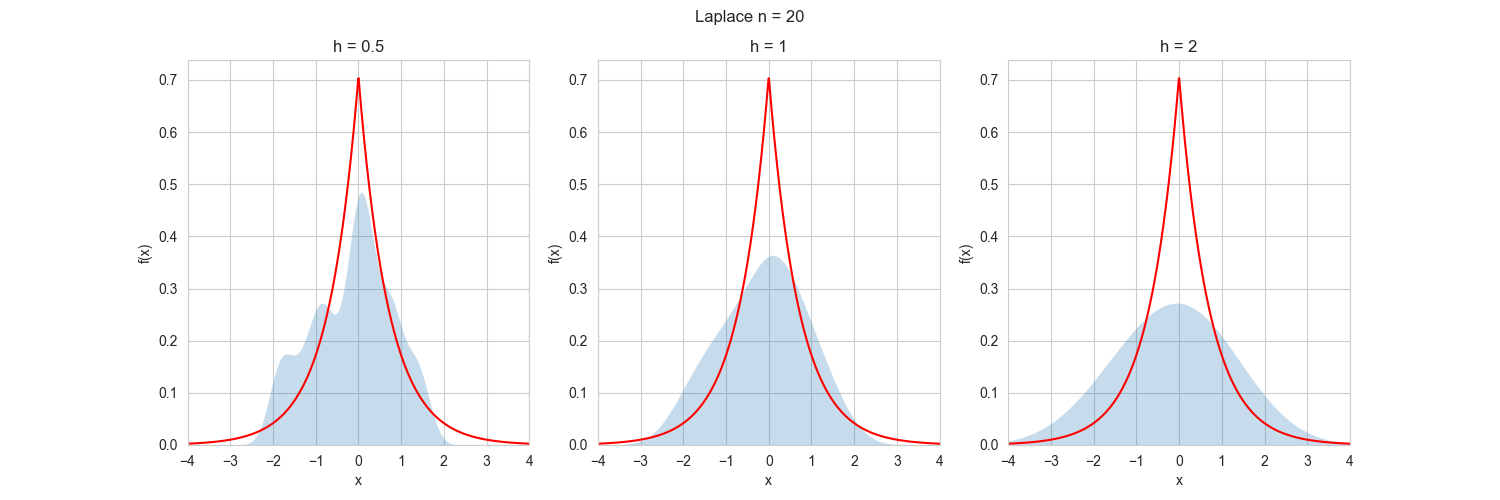
\includegraphics[scale=0.5]{figures/LaplaceNuclear20.png}
        \caption{Распределение Лапласа, n = 20}
        \label{fig:normal}
    \end{figure}
    
    \begin{figure}[H]
        \centering
        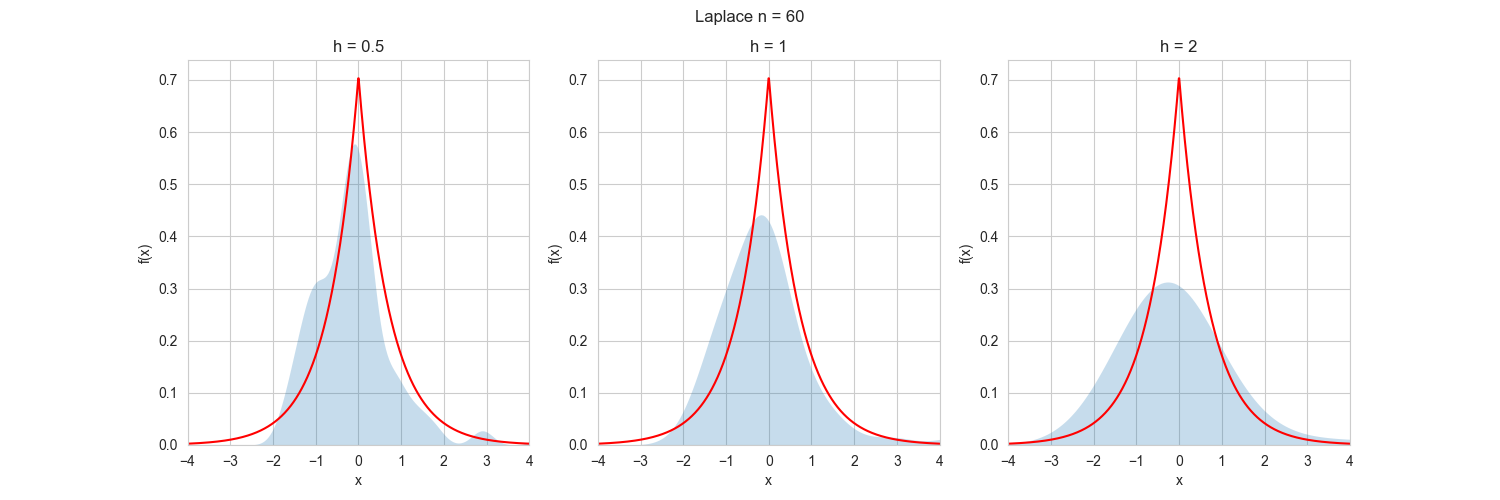
\includegraphics[scale=0.5]{figures/LaplaceNuclear60.png}
        \caption{Распределение Лапласа, n = 60}
        \label{fig:normal}
    \end{figure}
    
    \begin{figure}[H]
        \centering
        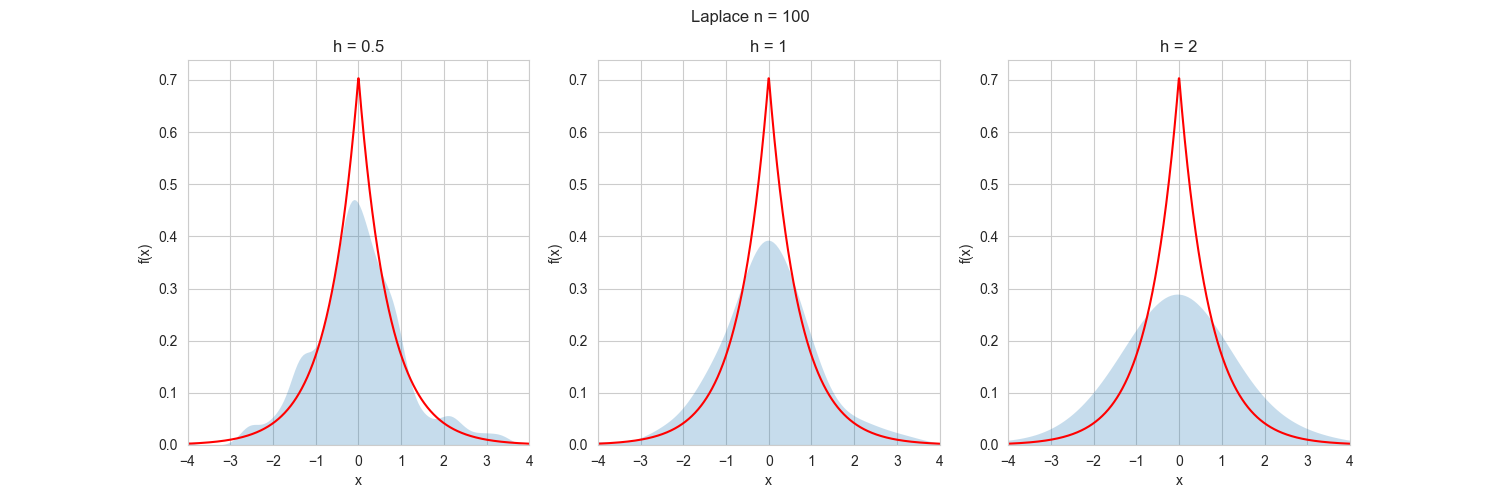
\includegraphics[scale=0.5]{figures/LaplaceNuclear100.png}
        \caption{Распределение Лапласа, n = 100}
        \label{fig:normal}
    \end{figure}
    
    \begin{figure}[H]
        \centering
        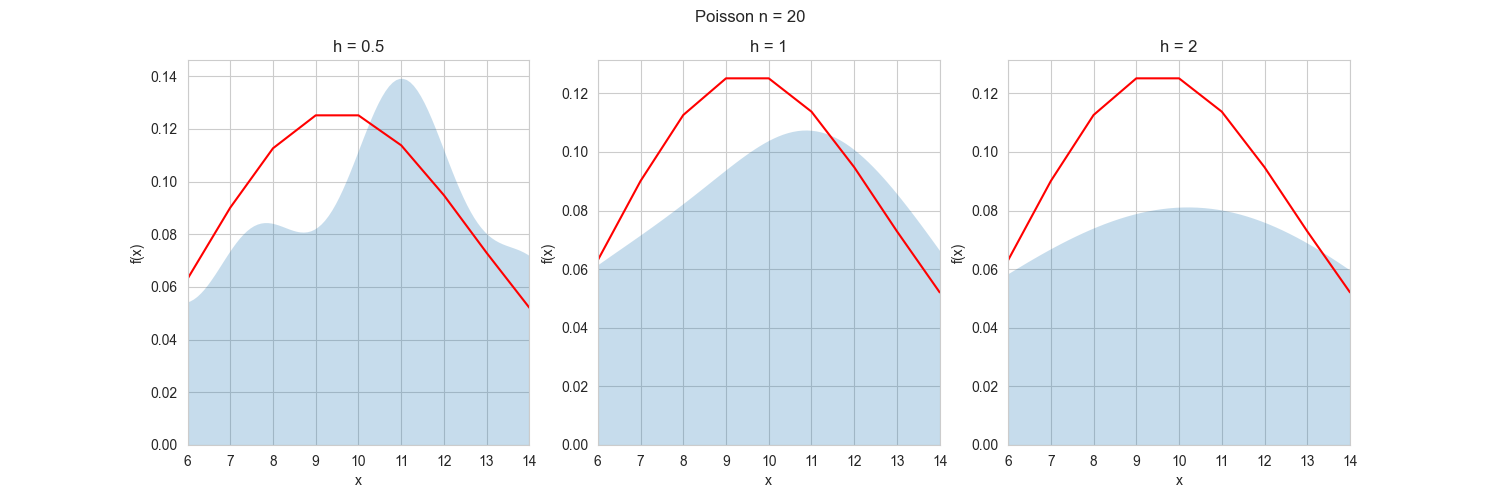
\includegraphics[scale=0.5]{figures/PoissonNuclear20.png}
        \caption{Распределение Пуассона, n = 20}
        \label{fig:normal}
    \end{figure}
    
    \begin{figure}[H]
        \centering
        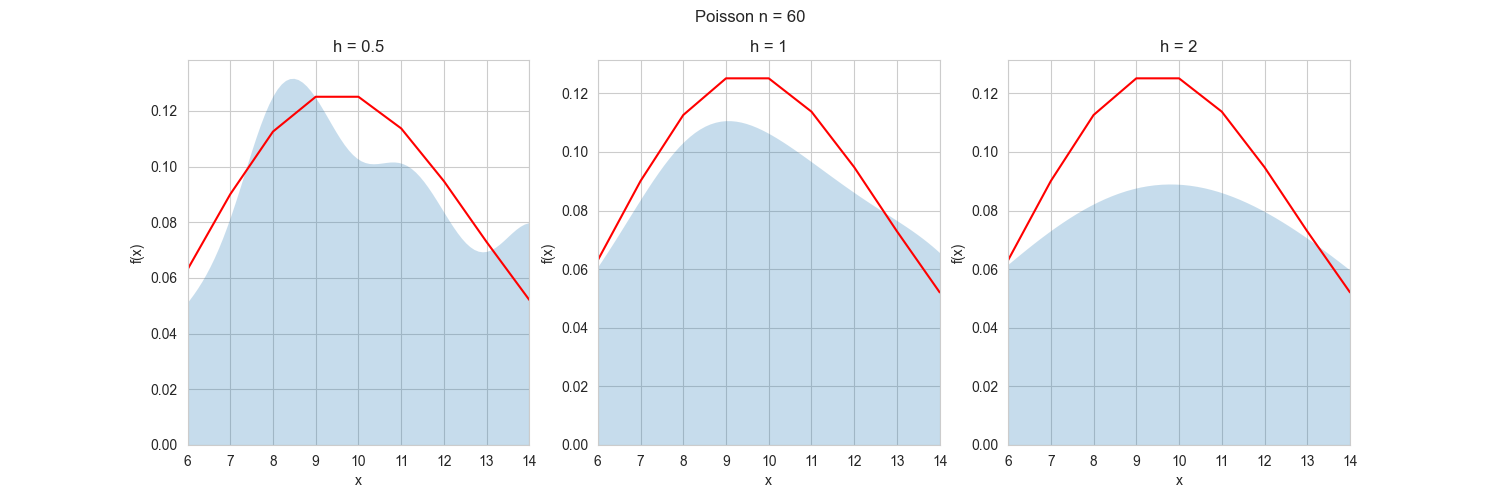
\includegraphics[scale=0.5]{figures/PoissonNuclear60.png}
        \caption{Распределение Пуассона, n = 60}
        \label{fig:normal}
    \end{figure}
    
    \begin{figure}[H]
        \centering
        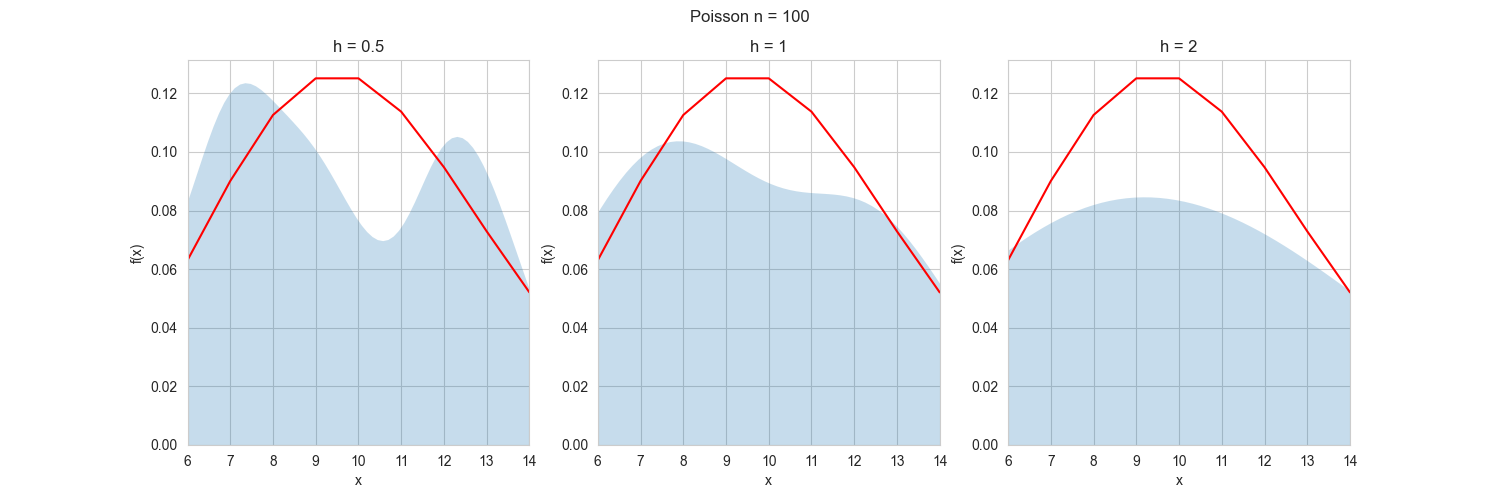
\includegraphics[scale=0.5]{figures/PoissonNuclear100.png}
        \caption{Распределение Пуассона, n = 100}
        \label{fig:normal}
    \end{figure}
    
    \begin{figure}[H]
        \centering
        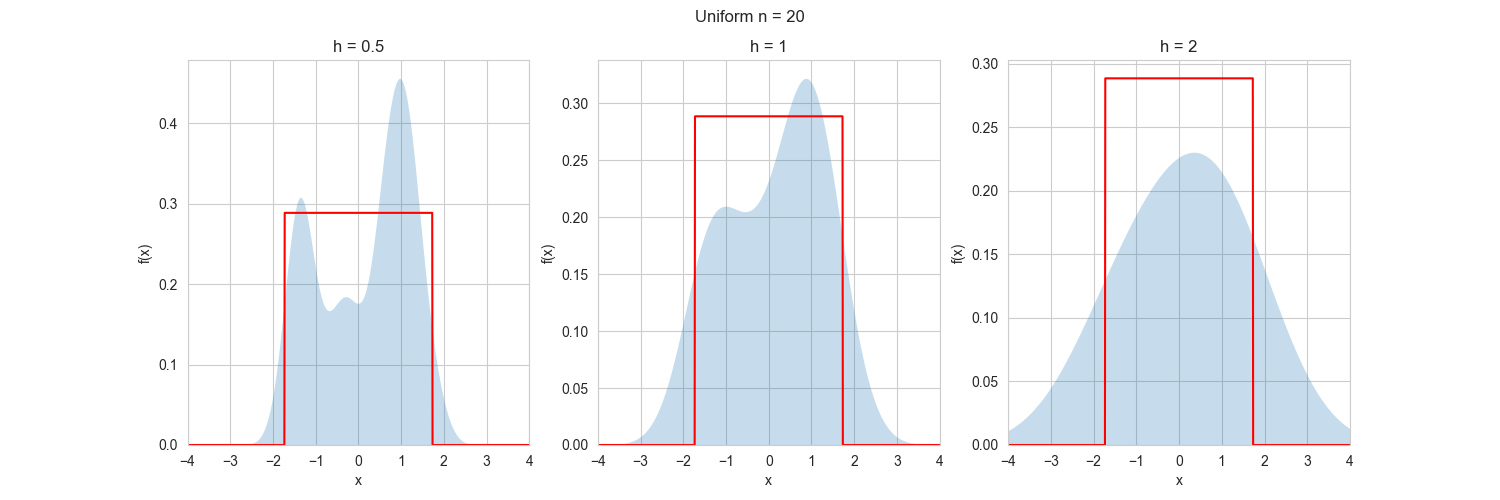
\includegraphics[scale=0.5]{figures/UniformNuclear20.png}
        \caption{Равномерное распределение, n = 20}
        \label{fig:normal}
    \end{figure}
    
    \begin{figure}[H]
        \centering
        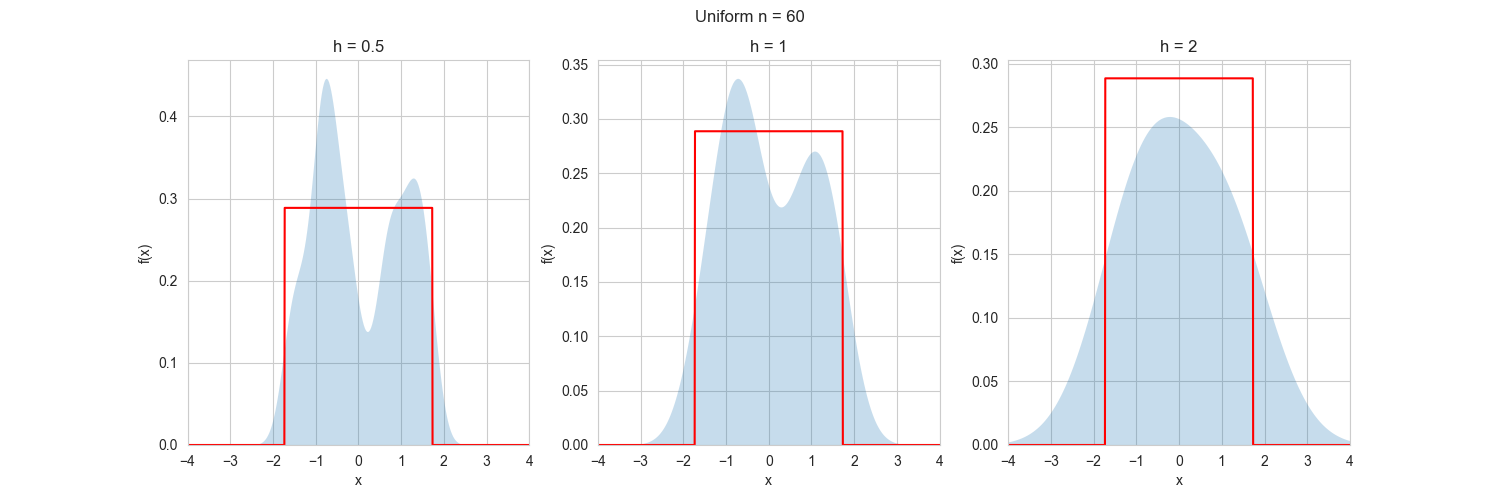
\includegraphics[scale=0.5]{figures/UniformNuclear60.png}
        \caption{Равномерное распределение, n = 60}
        \label{fig:normal}
    \end{figure}
    
    \begin{figure}[H]
        \centering
        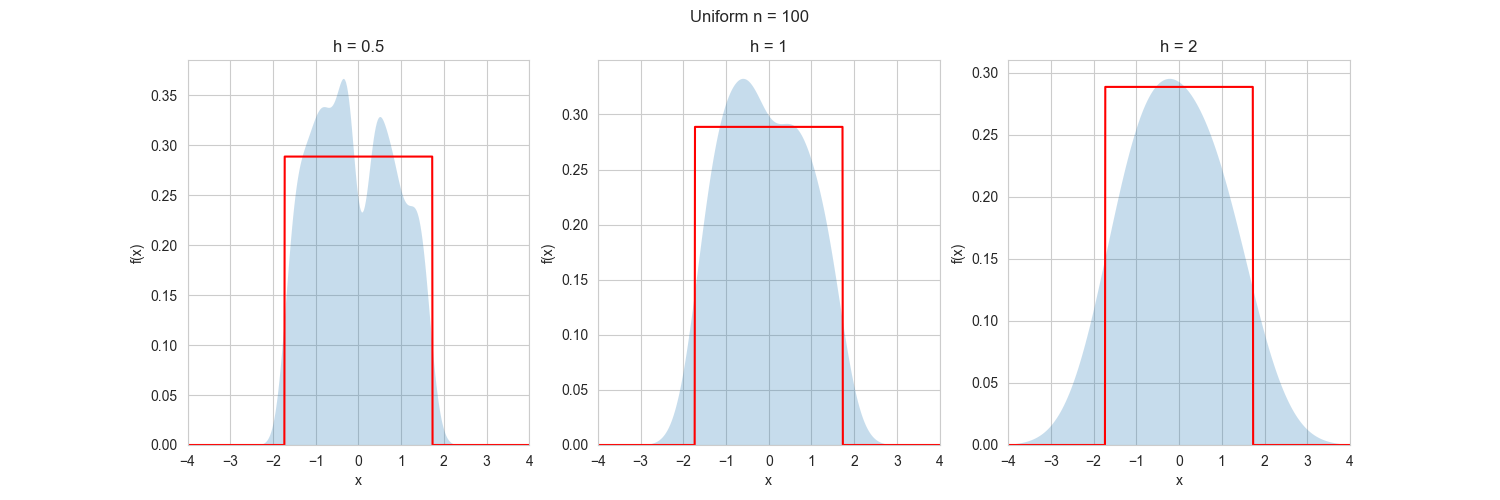
\includegraphics[scale=0.5]{figures/UniformNuclear100.png}
        \caption{Равномерное распределение, n = 100}
        \label{fig:normal}
    \end{figure}
\end{document}